\chapter{要素技術}
\label{technical_background}

本章では要素技術について述べる


\section{機械学習}

機械学習とは広義には, コンピューターが自動的にパターンを学習し人間による明示的な命令がなくとも
特定の課題を自動で実行する技術又はアルゴリズムのことである. 主に, 正解データを与えることによってパターンを学習する教師あり学習, データのまとまりや相関を求める教師なし学習と強化学習に分類される.


\section{深層学習}

深層学習とは脳が持つ脳神経系をソフトウェアで再現した人工ニューラルネット(ANN)を持つ機械学習アルゴリズムの一つである. 
人間の脳を模したパーセプトロンによる深層学習自体は1957年から提唱されていた. 4層以上のパーセプトロンでは過学習や勾配消失問題が発生しコンピューテーションコストも大きいためあまり普及しなかった.

\section{深層強化学習}

深層強化学習とは, 強化学習に深層学習を組み合わせた機械学習アルゴリズムである.
強化学習はエージェントとエージェントが動作する環境を定義し, 定義された環境下でエージェントへの報酬が最大化するように学習は行う.


\begin{figure}[H]
    \centering  % 図を真ん中に配置
    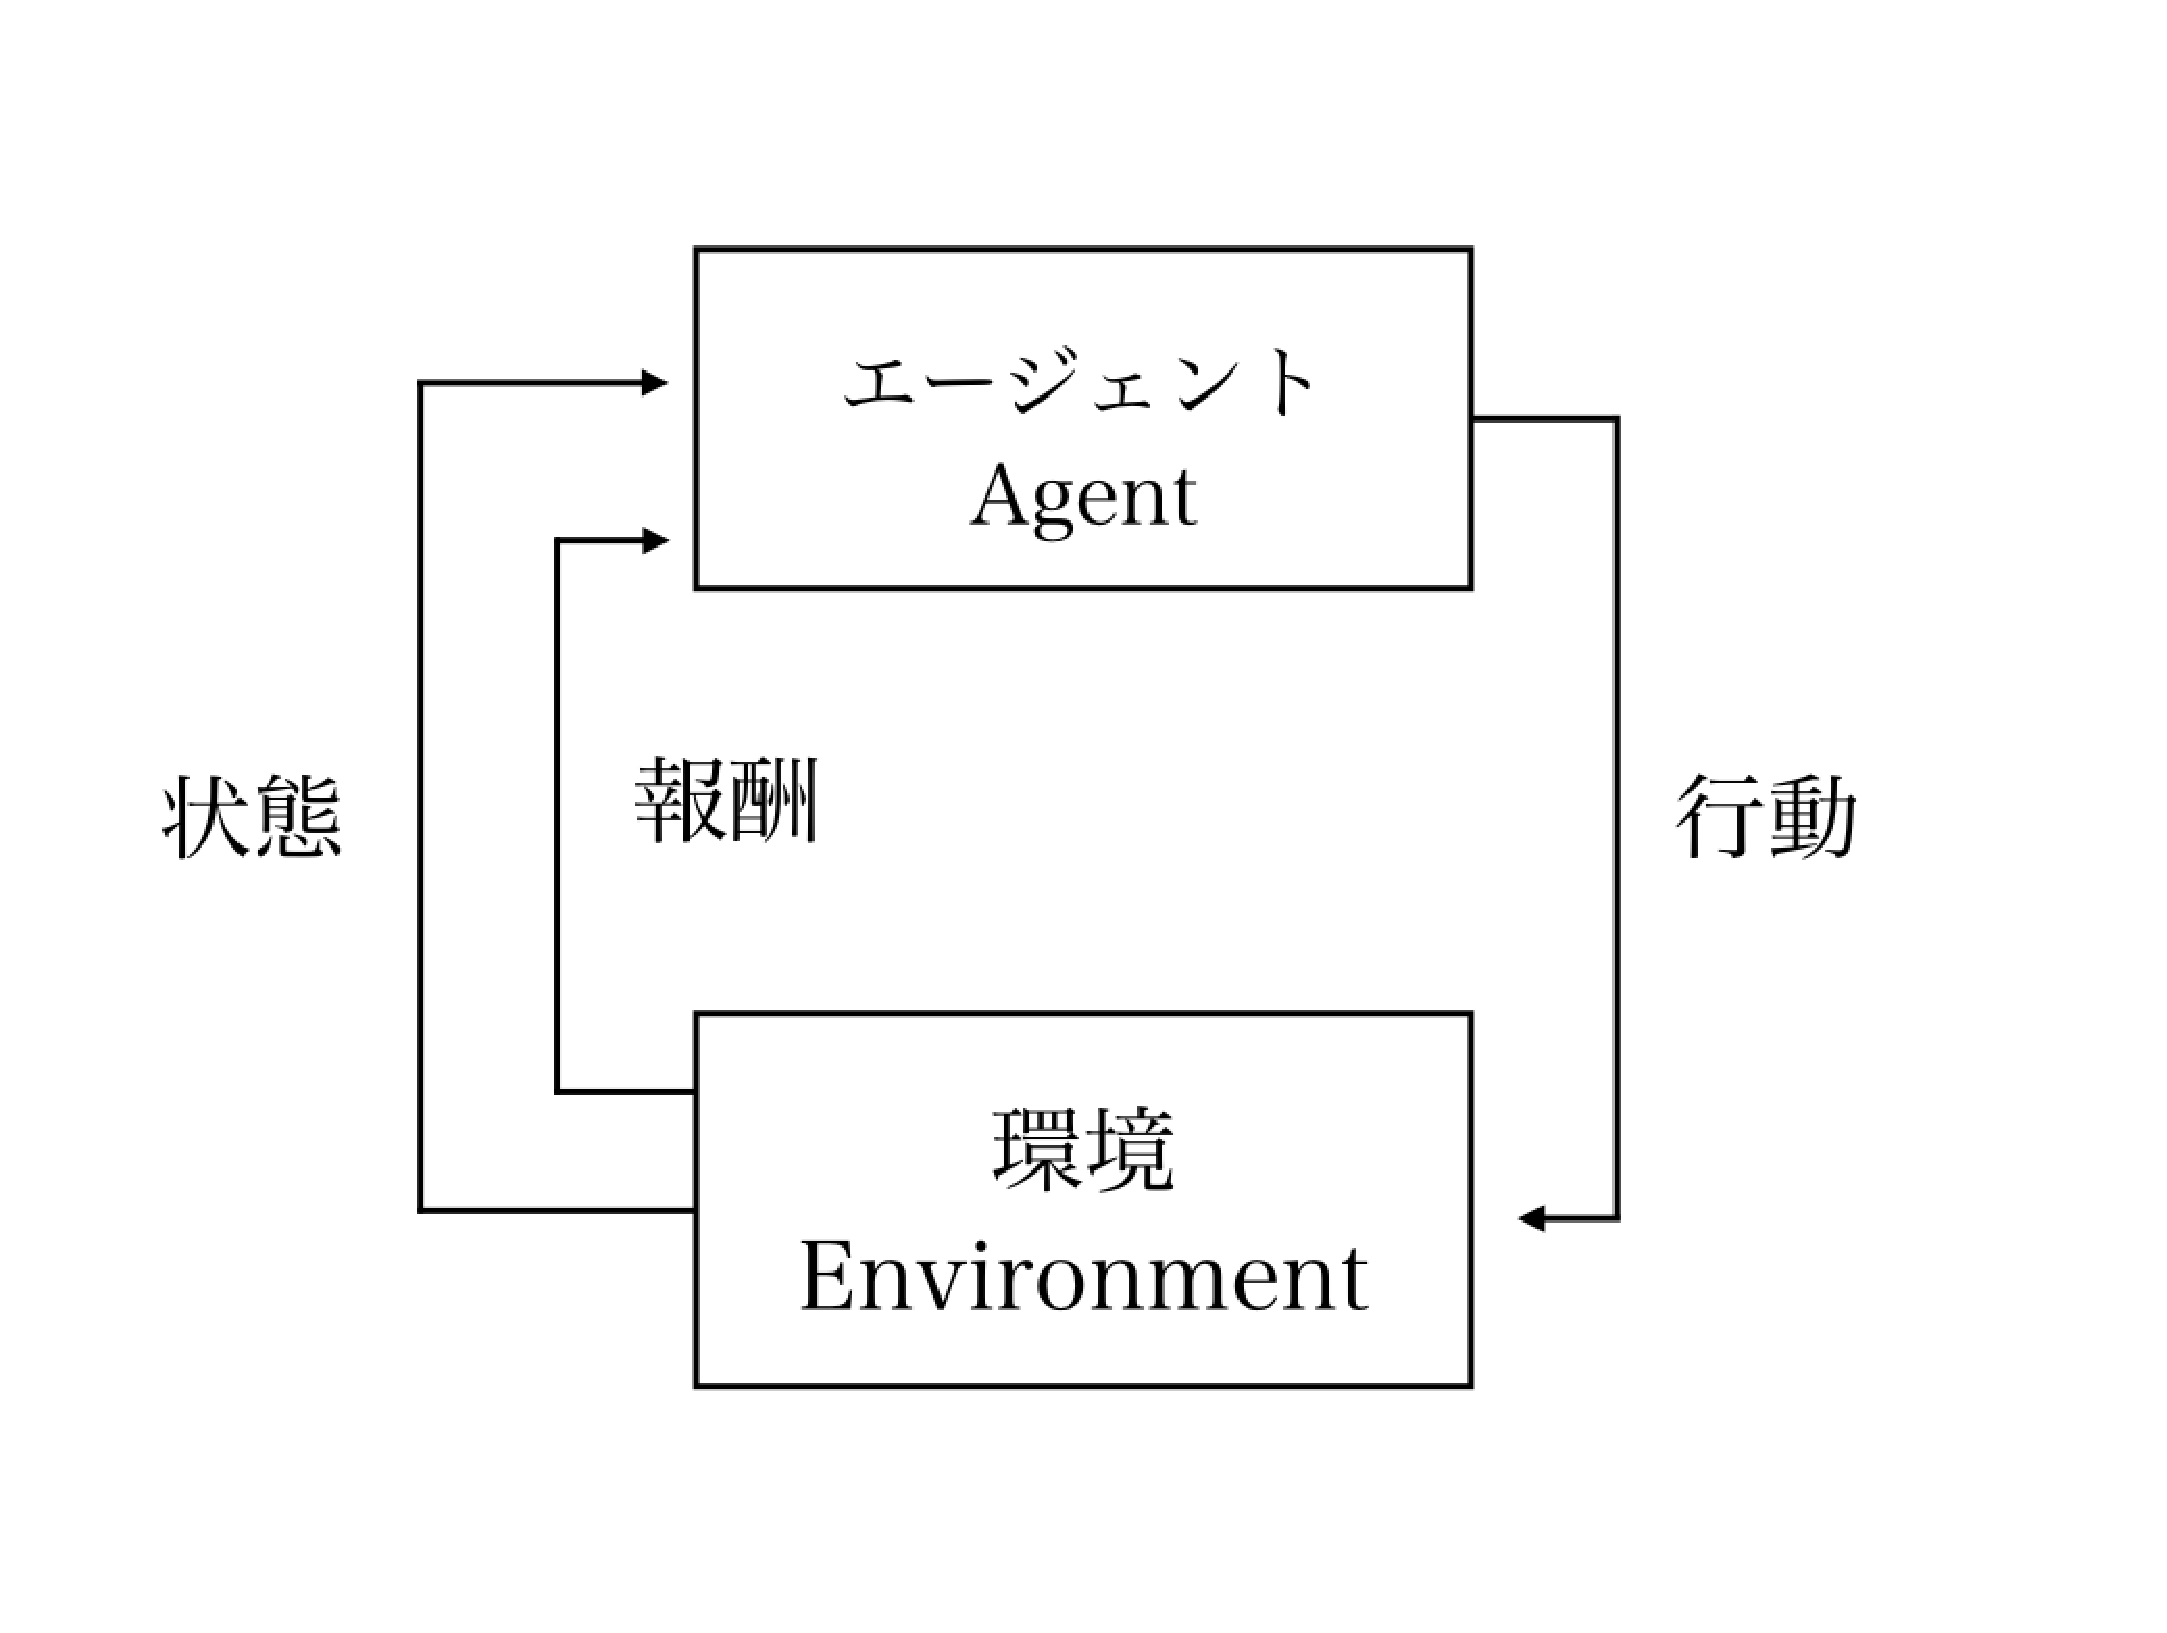
\includegraphics[clip,width = 12.0cm]{assets/reinforcement_learning.eps}
    \caption{強化学習による経路検索の結果}  \label{sample}
\end{figure}

\section{Deep Q Neural Network}

Deep Q Neural Network(DQN~\cite{DQN})はQ学習という強化学習における古典的なアルゴリズムを深層強化学習に応用したものである.


%%% Local Variables:
%%% mode: japanese-latex
%%% TeX-master: "../bthesis"
%%% End:
